\section{Experiment}
	Describes experimental settings:
	\begin{itemize}
		\item We use Stanford PoS tagger to produce input for parsing.
		\item Section 22 for experiments on effectiveness of A* and span features. Section 23 for the final results comparing to the others.
		\item Configuration of computer which runs the experiments.
	\end{itemize}
	% Please add the following required packages to your document preamble:
% \usepackage{multirow}
\begin{table*}[t]
	\caption{\label{devEx1} The results of experiment comparing between A* parser with different beam search systems}
	\begin{center}
		\begin{tabular}{|c|c|c|c|c|c|c|c|}
			\hline
			\multicolumn{2}{|c|}{\multirow{3}{*}{\textbf{System}}} & \multicolumn{3}{c|}{\textbf{Baseline Features}}                                                                                & \multicolumn{3}{c|}{\textbf{Span Features}}                                                                                    \\ \cline{3-8} 
			\multicolumn{2}{|c|}{}                                 & \multicolumn{2}{c|}{\textit{F-score}} & \multirow{2}{*}{\textit{\begin{tabular}[c]{@{}c@{}}Speed\\ (sentence/s)\end{tabular}}} & \multicolumn{2}{c|}{\textit{F-score}} & \multirow{2}{*}{\textit{\begin{tabular}[c]{@{}c@{}}Speed\\ (sentence/s)\end{tabular}}} \\ \cline{3-4} \cline{6-7}
			\multicolumn{2}{|c|}{}                                 & \textit{non-DP}     & \textit{DP}     &                                                                                        & \textit{non-DP}     & \textit{DP}     &                                                                                        \\ \hline
			\multirow{3}{*}{Beam Search}        & beam = 16        & 89.1                & 90.1            & 34.6                                                                                   & 88.6                & 89.9            & 31.9                                                                                   \\ \cline{2-8} 
			& beam = 32        & 89.6               & 89.9            & 20                                                                                     & 89.3                & 90.2            & 17                                                                                     \\ \cline{2-8} 
			& beam = 64        & 89.7                & 90.2            & 10.6                                                                                   & 89.6               & 90.2           & 9.1                                                                                    \\ \hline
			\multicolumn{2}{|c|}{A* Search}                        & N/A                 & N/A             & N/A                                                                                    & N/A                 & 90.7            & 13.6                                                                                   \\ \hline
			\multicolumn{2}{|c|}{Best First Search}                & N/A                 & N/A             & N/A                                                                                    & N/A                 & 90.7            & 1.12                                                                                   \\ \hline
		\end{tabular}
	\end{center}
\end{table*}
	% Please add the following required packages to your document preamble:
% \usepackage{multirow}
\begin{table*}[t]
	\caption{\label{devEx1} The results of experiment comparing between A* parser with different beam search systems}
	\begin{center}
		\begin{tabular}{|c|c|c|c|c|c|c|c|}
			\hline
			\multicolumn{2}{|c|}{\multirow{3}{*}{\textbf{System}}} & \multicolumn{3}{c|}{\textbf{Baseline Features}}                                                                                & \multicolumn{3}{c|}{\textbf{Span Features}}                                                                                    \\ \cline{3-8} 
			\multicolumn{2}{|c|}{}                                 & \multicolumn{2}{c|}{\textit{F-score}} & \multirow{2}{*}{\textit{\begin{tabular}[c]{@{}c@{}}Speed\\ (sentence/s)\end{tabular}}} & \multicolumn{2}{c|}{\textit{F-score}} & \multirow{2}{*}{\textit{\begin{tabular}[c]{@{}c@{}}Speed\\ (sentence/s)\end{tabular}}} \\ \cline{3-4} \cline{6-7}
			\multicolumn{2}{|c|}{}                                 & \textit{non-DP}     & \textit{DP}     &                                                                                        & \textit{non-DP}     & \textit{DP}     &                                                                                        \\ \hline
			\multirow{3}{*}{Beam Search}        & beam = 16        & 89.1                & 90.1            & 34.6                                                                                   & 88.6                & 89.9            & 31.9                                                                                   \\ \cline{2-8} 
			& beam = 32        & 89.6               & 89.9            & 20                                                                                     & 89.3                & 90.2            & 17                                                                                     \\ \cline{2-8} 
			& beam = 64        & 89.7                & 90.2            & 10.6                                                                                   & 89.6               & 90.2           & 9.1                                                                                    \\ \hline
			\multicolumn{2}{|c|}{A* Search}                        & N/A                 & N/A             & N/A                                                                                    & N/A                 & 90.7            & 13.6                                                                                   \\ \hline
			\multicolumn{2}{|c|}{Best First Search}                & N/A                 & N/A             & N/A                                                                                    & N/A                 & 90.7            & 1.12                                                                                   \\ \hline
		\end{tabular}
	\end{center}
\end{table*}
\subsection{Speed and Accuracy Comparison}
	\begin{itemize}
		\item Comparing search quality between difference A* heuristic on span features. (Figure \ref{devExFig1})
		\item Comparing search quality between A* parser with beam search parser with different beam size on span features. (Figure \ref{devExFig2})
		\item Total performance comparison between our A* parser with beam search on span features and Zhang's baseline in both accuracy and speed.
	\end{itemize}
	
	\begin{figure}
	\begin{center}
		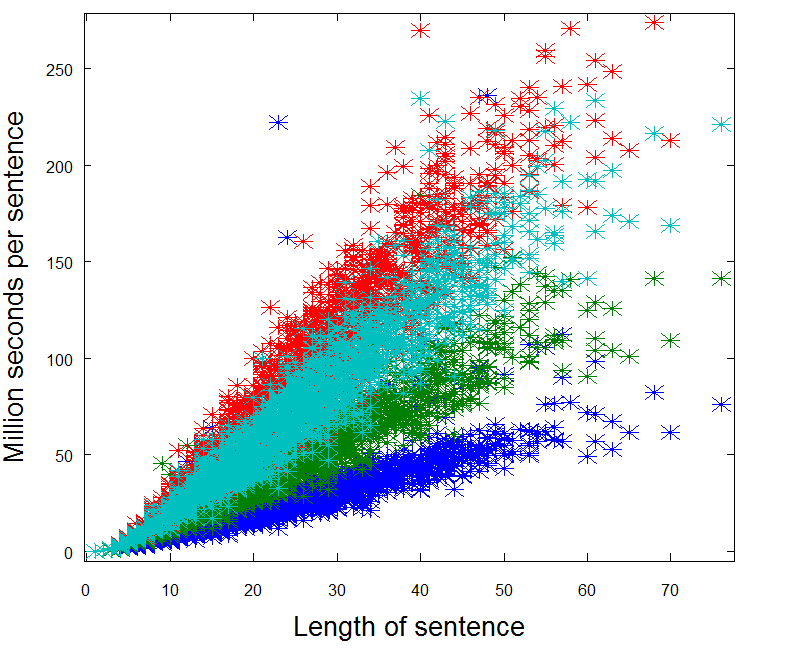
\includegraphics[scale=0.35]{Figures/SpeedAndAccuracyComparison2.png}
		\caption{\label{devExFig2} The parsing time comparison between A* and beam search. The blue one is beam size = 16, the green one is beam size = 32, the red one is beam size = 64, and the cyan one is our hybrid A*.}
	\end{center}
\end{figure}
\subsection{Final Results}
	The results of final experiment to show that our parser can achieve a state-of-the-art performance with only simplified feature template.
	\begin{table*}[t]
	\caption{\label{finalEx} The final results on section 23 of English Penn Treebank}
	\begin{center}
		\begin{tabular}{l|c|c|c|c}
			\hline
			\textbf{System} & \textbf{\begin{tabular}[c]{@{}c@{}}Speed\\ (sentence/s)\end{tabular}} & \textbf{LR} & \textbf{LP} & \textbf{F1} \\ \hline
			Johnson and Charniak (2005) & 2.1 & 91.2 & 91.8 & 91.5 \\
			Mc Closky (2006) & 1.2 & 92.2 & 92.6 & 92.4 \\
			Berkeley parser & 6.1 & 90.1 & 90.3 & 90.2 \\
			Stanford parser (2014) & 3.3 & 90.3 & 90.7 & 90.5 \\
			Zhang Yue (2012) - baseline & 107.5 & 90.0 & 89.9 & 89.9 \\
			Zhang Yue(2012) - baseline+padding & 93.4 & 90.2 & 90.7 & 90.4 \\
			Zhang Yue(2012) - baseline+padding+semi & 47.6 & 91.1 & 91.5 & 91.3 \\
			Sagae \& Lavie (2005)* & 3.7 & 86.0 & 86.1 & 86.0 \\
			Sagae \& Lavie(2006)* & 2.2 & 88.1 & 87.8 & 87.9 \\
			\textbf{This paper} & \textbf{13.6} & \textbf{90.9} & \textbf{91.2} & \textbf{91.1} \\
			\hline
		\end{tabular}
	\end{center}
\end{table*}
		
	